% Auto-generated by scripts/benchmark_baseline.py
% Append to IEEE Computer manuscript Appendix B (Benchmarks).

\begin{figure}[t]
\centering
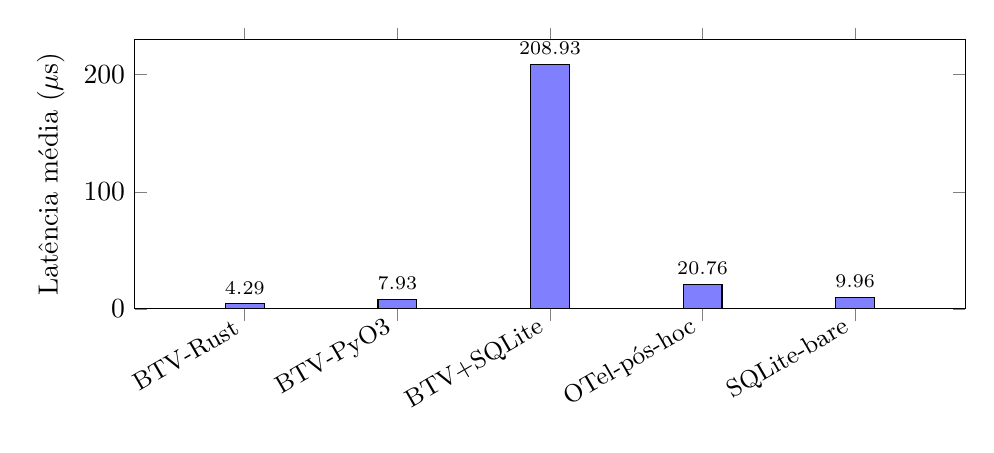
\begin{tikzpicture}
\begin{axis}[
    ybar,
    bar width=14pt,
    width=\columnwidth,
    height=5cm,
    ylabel={Latência média ($\mu$s)},
    symbolic x coords={BTV-Rust, BTV-PyO3, BTV+SQLite, OTel-pós-hoc, SQLite-bare},
    xtick=data,
    x tick label style={rotate=30,anchor=east,font=\small},
    nodes near coords,
    nodes near coords style={font=\scriptsize},
    enlarge x limits=0.18,
    ymin=0,
]
\addplot[fill=blue!50] coordinates {
    (BTV-Rust, 4.29)
    (BTV-PyO3, 7.93)
    (BTV+SQLite, 208.93)
    (OTel-pós-hoc, 20.76)
    (SQLite-bare, 9.96)
};
\end{axis}
\end{tikzpicture}
\caption{Latência MÉDIA por implementação ($N=5{,}000$ para Python; $N=100$ para Rust/Criterion). Todas as barras plotam médias (Criterion fornece média, não percentis — OS-08/F8); ver Tabela~\ref{tab:bench-stats}.}
\label{fig:bench-baseline}
\end{figure}

\begin{table}[t]
\centering
\caption{Estatísticas de benchmark por implementação.}
\label{tab:bench-stats}
\small
\begin{tabular}{lrrrr}
\toprule
Implementação & média ($\mu$s) & stdev ($\mu$s) & ops/s & estatística de latência \\
\midrule
BTV-Rust-native & 4.29 & 18.08 & 233260 & mean (Criterion) \\
BTV-PyO3 & 7.93 & 3.46 & 126111 & measured percentiles (perf_counter, single-threaded) \\
BTV-Rust+SQLite WAL+FULL & 208.93 & 120.41 & 4786 & mean (Criterion) \\
OpenTelemetry pós-hoc & 20.76 & 31.45 & 48164 & measured percentiles (perf_counter, single-threaded) \\
SQLite ACID bare & 9.96 & 4.25 & 100442 & measured percentiles (perf_counter, single-threaded) \\
\bottomrule
\end{tabular}
\end{table}
